\epigraph{\textit{"Let's change as little as possible"}}

\paragraph{Abstract} A series of top cathode perovskite solar cells have been fabricated with slightly different layers thicknesses. We verified that these variations affected as little as possible the rest of the solar cell stack, so that we could unequivocally relate the observations to the changes. The characterization via current-voltage sweeps and photophysical techniques allowed us to study the charge distribution in these devices.

\paragraph{Publications} Part of this chapter has been published in \fullcite{Gelmetti2017}.

\section{Introduction}

	\paragraph{Disentangling parameters' impact} Perovskite synthesis is a very easy and very fragile process at the same time. When varying a fabrication parameter, for example during an optimization, it is quite likely to provoke a "butterfly effect" with the resulting device differing from the reference one by much more than the characteristic under study. A principal component analysis of the fabrication parameters would be needed for a rational optimization, but such a complex procedure is further hindered by the difficulty of identifying all relevant contributions.

	\paragraph{Varying the thickness} In this study we vary a set of parameters that hopefully have a foreseeable relation with the resulting device structure: The spin coating speed for each layer. The effect of this variation should just affect the layers thicknesses with a minor influence on the other device physical features. This will allow us to univocally relate each layer thickness variation to the characterization results variation. The complete devices were studied by means of current-voltage sweeps, \acr{ce}, \acr{tpv}, and \acr{dc}.

	\paragraph{The devices} The chosen architecture was a top cathode \gls{ito}/\gls{pedotpss}/\gls{mapi}/\gls{pcbm70}/\ch{Ag} device (fabrication described in \cpagerefrange{methods_top}{methods_top_end}) and the layers whose thickness was independently varied are the \gls{pedotpss} (\gls{htm}), the \gls{mapi} (absorber), and the \gls{pcbm70} (\gls{etm}).

\section{Interpretation of \gls{jsc} and \gls{ff} from Current-Voltage Sweeps}

\section{Interpretation of Transient PhotoCurrent}\label{interpretation_tpc}

\section{Interpretation of Differential Capacitance}\label{interpretation_dc}

	A common commercial capacitor has a capacitance which is constant regardless to the voltage applied to it, as can be seen in \cref{fig:cap_voltage_dependence_commercial}.

	\begin{figure}%[!hbtp]%
		\centering
		\begin{subfigure}[t]{0.45\textwidth}
			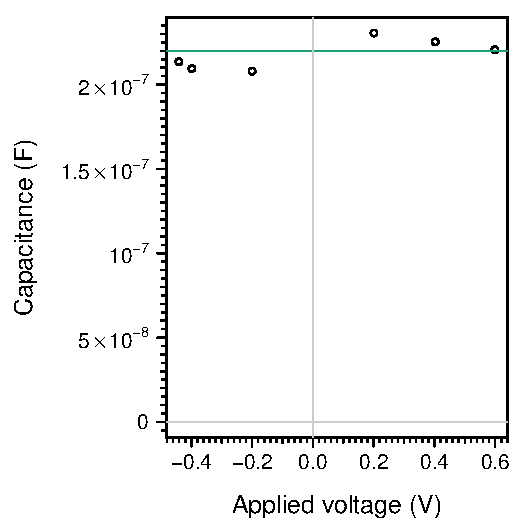
\includegraphics[width=1\textwidth]{cap_voltage_dependence/reference220nF/reference220nF.pdf}
			\subcaption{Commercial \SI{220}{\nano\F} capacitor.}\label{fig:cap_voltage_dependence_commercial}
		\end{subfigure}
		\qquad
		\begin{subfigure}[t]{0.45\textwidth}
			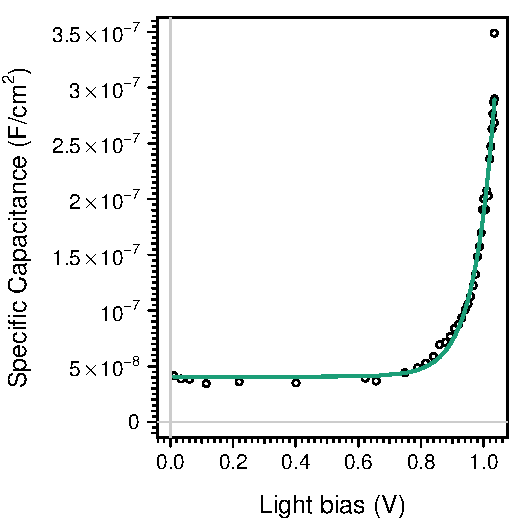
\includegraphics[width=1\textwidth]{cap_voltage_dependence/TAE-1_ig94-1559-1/DC-capacitance-TAE-1_ig94-1559-1.pdf}
			\subcaption{Perovskite solar cell.}\label{fig:cap_voltage_dependence_tae1}
		\end{subfigure}
		\mycaption[Capacitance dependence on applied voltage.]{In (a) the capacitance of a commercial capacitor is reported, it was measured using \acr{ce} with applied voltage bias instead of the classical light bias used for solar cells. The capacitance is obtained as the extracted charge over the applied voltage prior to short circuiting. In (b) the typical capacitance versus voltage profile of a \gls{fto}/\dTiOtwo/\mpTiOtwo/\acr{csfamapbibr}/\tae1/Au device is shown. In this case the indicated voltage is originated by various illumination intensities at open circuit prior to short circuiting.}\label{fig:cap_voltage_dependence}
	\end{figure}

\section{Interpretation of Transient PhotoVoltage Referenced to Differential Capacitance}\label{interpretation_tpvdc}


\section{Varying \gls{mapi} Thickness (Absorber Layer)}


\section{Varying \gls{pcbm70} Thickness (\gls{etm} Layer)}
\section{Varying \gls{pedotpss} Thickness (\gls{htm} Layer)}
\section{Conclusions}
\section{Critical Assessment}